\documentclass[../main]{subfiles}
\begin{document}
\setcounter{secnumdepth}{3}
    \chapter{実験}
    \section{実験目的}
        本研究で提案した全天球カメラ画像に基づく通路分類手法の有効性をロボットを用いた実環境での実験により検証する.
    \section{実験の概要}
        提案した通路分類手法の有効性をロボットを用いた実環境での実験により検証する.
        実験環境は\fref{figure::3floor_map}に示す千葉工業大学津田沼キャンパス2号館3階の廊下とした.
        \begin{figure}[H]
         \centering
         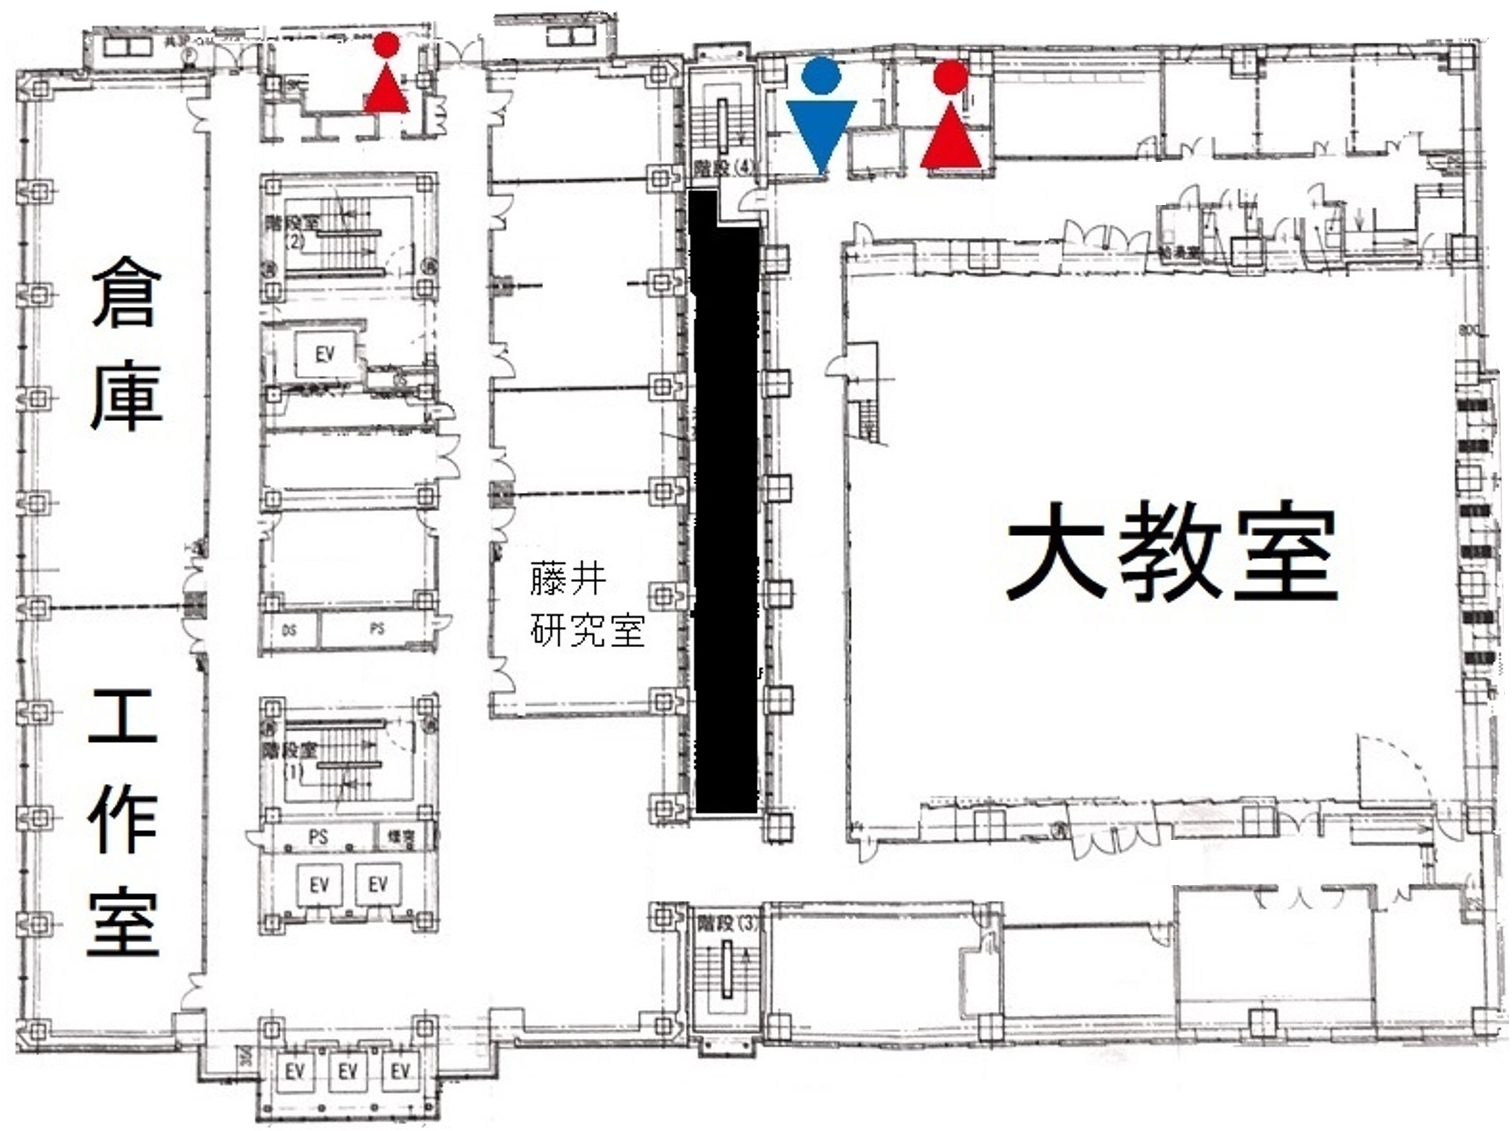
\includegraphics[width=15cm]{../images/MAP_Tsudanuma2-3.png}
         \caption{Experiment environment}
         \label{figure::3floor_map}
        \end{figure}

    \section{実験装置}
        実験には本研究室で開発をしているORNE-αを用いた.また,機体とその構成,使用したPCのスペックをそれぞれ
        \fref{figure::robot_image},\tref{table::robot_spec},\tref{table::pc_spec}に示す.

        \begin{figure}[H]
        \centering
        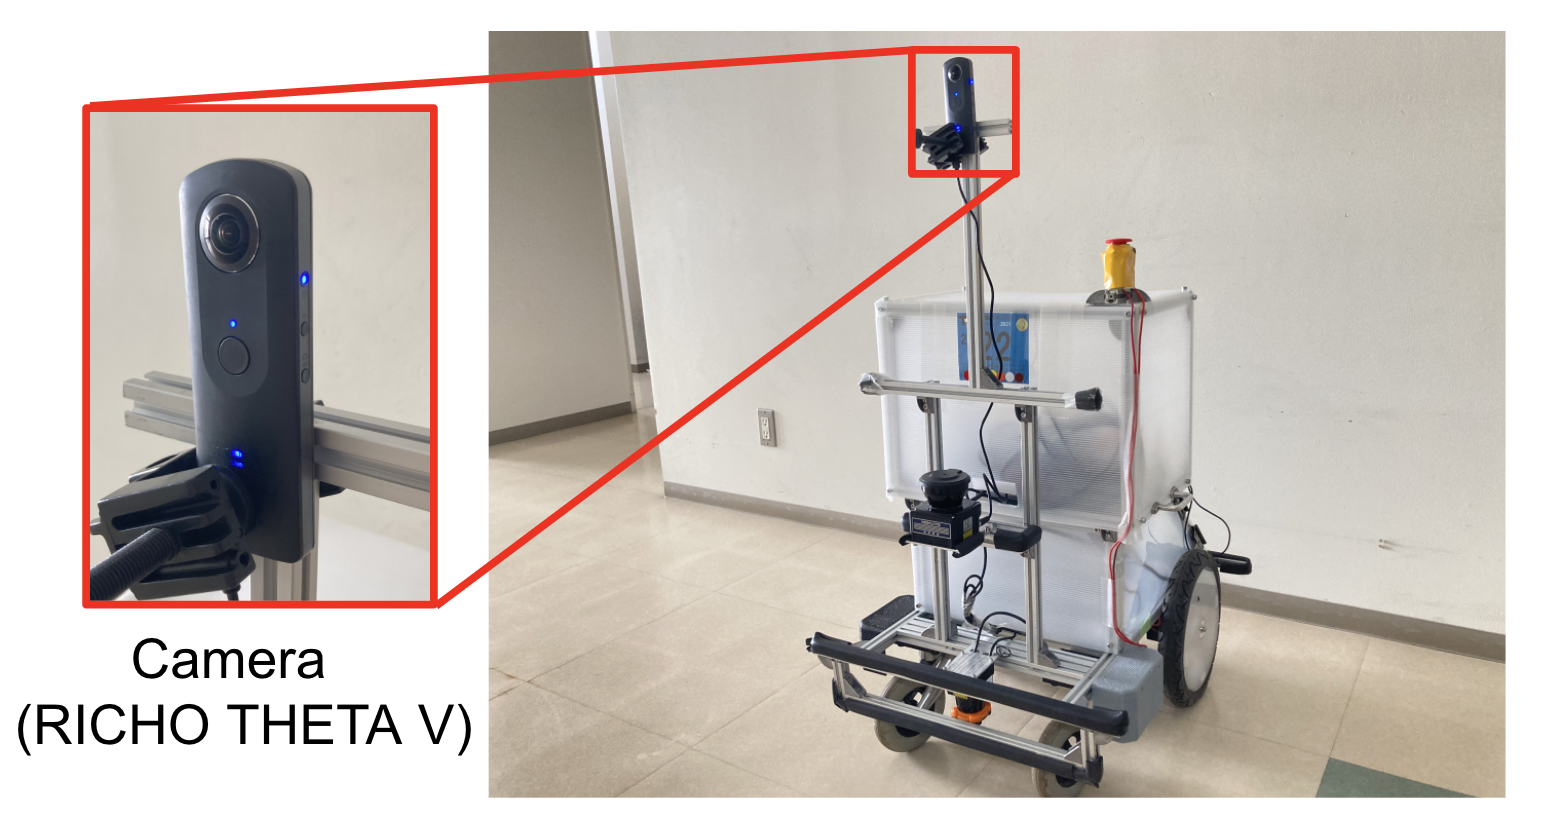
\includegraphics[width=7cm]{../images/experimental_machine_wide.png}
        \caption{ORNE-α}
        \label{figure::robot_image}
        \end{figure}

        \begin{table}[H]
         \centering
         \caption{Specification of PC}
         \begin{tabular}{l|l} \hline
         \multicolumn{1}{c|}{CPU} & \multicolumn{1}{c}{Core i7-9750H(Intel)} \\ \hline
         \multicolumn{1}{c|}{RAM} & \multicolumn{1}{c}{16GB} \\ \hline
         \multicolumn{1}{c|}{GPU} & \multicolumn{1}{c}{RTX 2070 Max-Q} \\ \hline
         \end{tabular}
         \label{table::pc_spec}
        \end{table}

        \begin{table}[H]
            \centering
            \caption{Specification of ORNE-α}
            \begin{tabular}{l|l}\hline
            \multicolumn{1}{c|}{item}                                                              & \multicolumn{1}{c}{ORNE-α}                              \\ \hline
            \multicolumn{1}{c|}{Depth{[}mm{]}}                                                     & \multicolumn{1}{c}{710} \\ \hline
            \multicolumn{1}{c|}{Wide{[}mm{]}}                                                      & \multicolumn{1}{c}{560}                                 \\ \hline
            \multicolumn{1}{c|}{Height{[}mm{]}}                                                    & \multicolumn{1}{c}{810}                                  \\ \hline
            \multicolumn{1}{c|}{Weight{[}kg{]}}                                                    & \multicolumn{1}{c}{20}                                   \\ \hline
            \multicolumn{1}{c|}{\begin{tabular}[c]{@{}c@{}}Wheel diameter\\ {[}mm{]}\end{tabular}} & \multicolumn{1}{c}{304}                                   \\ \hline
            \multicolumn{1}{c|}{Battery}                                                           & \multicolumn{1}{c}{LONG WP12-12 × 2}                      \\ \hline
            \multicolumn{1}{c|}{Motor}                                                             & \multicolumn{1}{c}{Oriental motor TF-M30-24-3500-G15L/R}  \\ \hline
            \multicolumn{1}{c|}{Spherical camera}                                                  & \multicolumn{1}{c}{RICOH THETA V}  \\ \hline
            \end{tabular}
            \label{table::robog_spec}
            \end{table}

    \section{全天球カメラを用いた通路分類の検証}
        \subsection{実験方法}
        全天球カメラを取り付けた実ロボットを実験環境の25地点に移動させ,各地点で全天球カメラにより取得した画像データを用いて,
        提案手法により通路の特徴分類ができるかどうかを検証する.
        \fref{figure::experiment_point}の丸い図形により示す実験環境の25箇所にロボットを移動させ,
        各地点で取得した全天球カメラ画像から提案した手法により通路の分類を行う.
        また,先行研究で述べられた通り,人が道案内により移動する際には,向いている方向の情報も必要としているため,
        同一箇所においてもロボットの向いている方向により分類される通路の特徴が変化する場合,ロボットの向きを変え,各向きを向いた状態
        を1例とし,正しく通路分類が行えるかどうか検証する.
        本実験の環境では,同一箇所においてもロボットの向きで通路の特徴が異なる箇所が●箇所存在したため,全●例の通路分類ができるかを検証する.
        ロボットの移動にはジョイスティックコントローラーを使用する.実験の条件として,突き当たりと通路の判定する境界は,
        5m先が行き止まりかどうかにより判断を行うこととする.

        \begin{figure}[H]
         \centering
         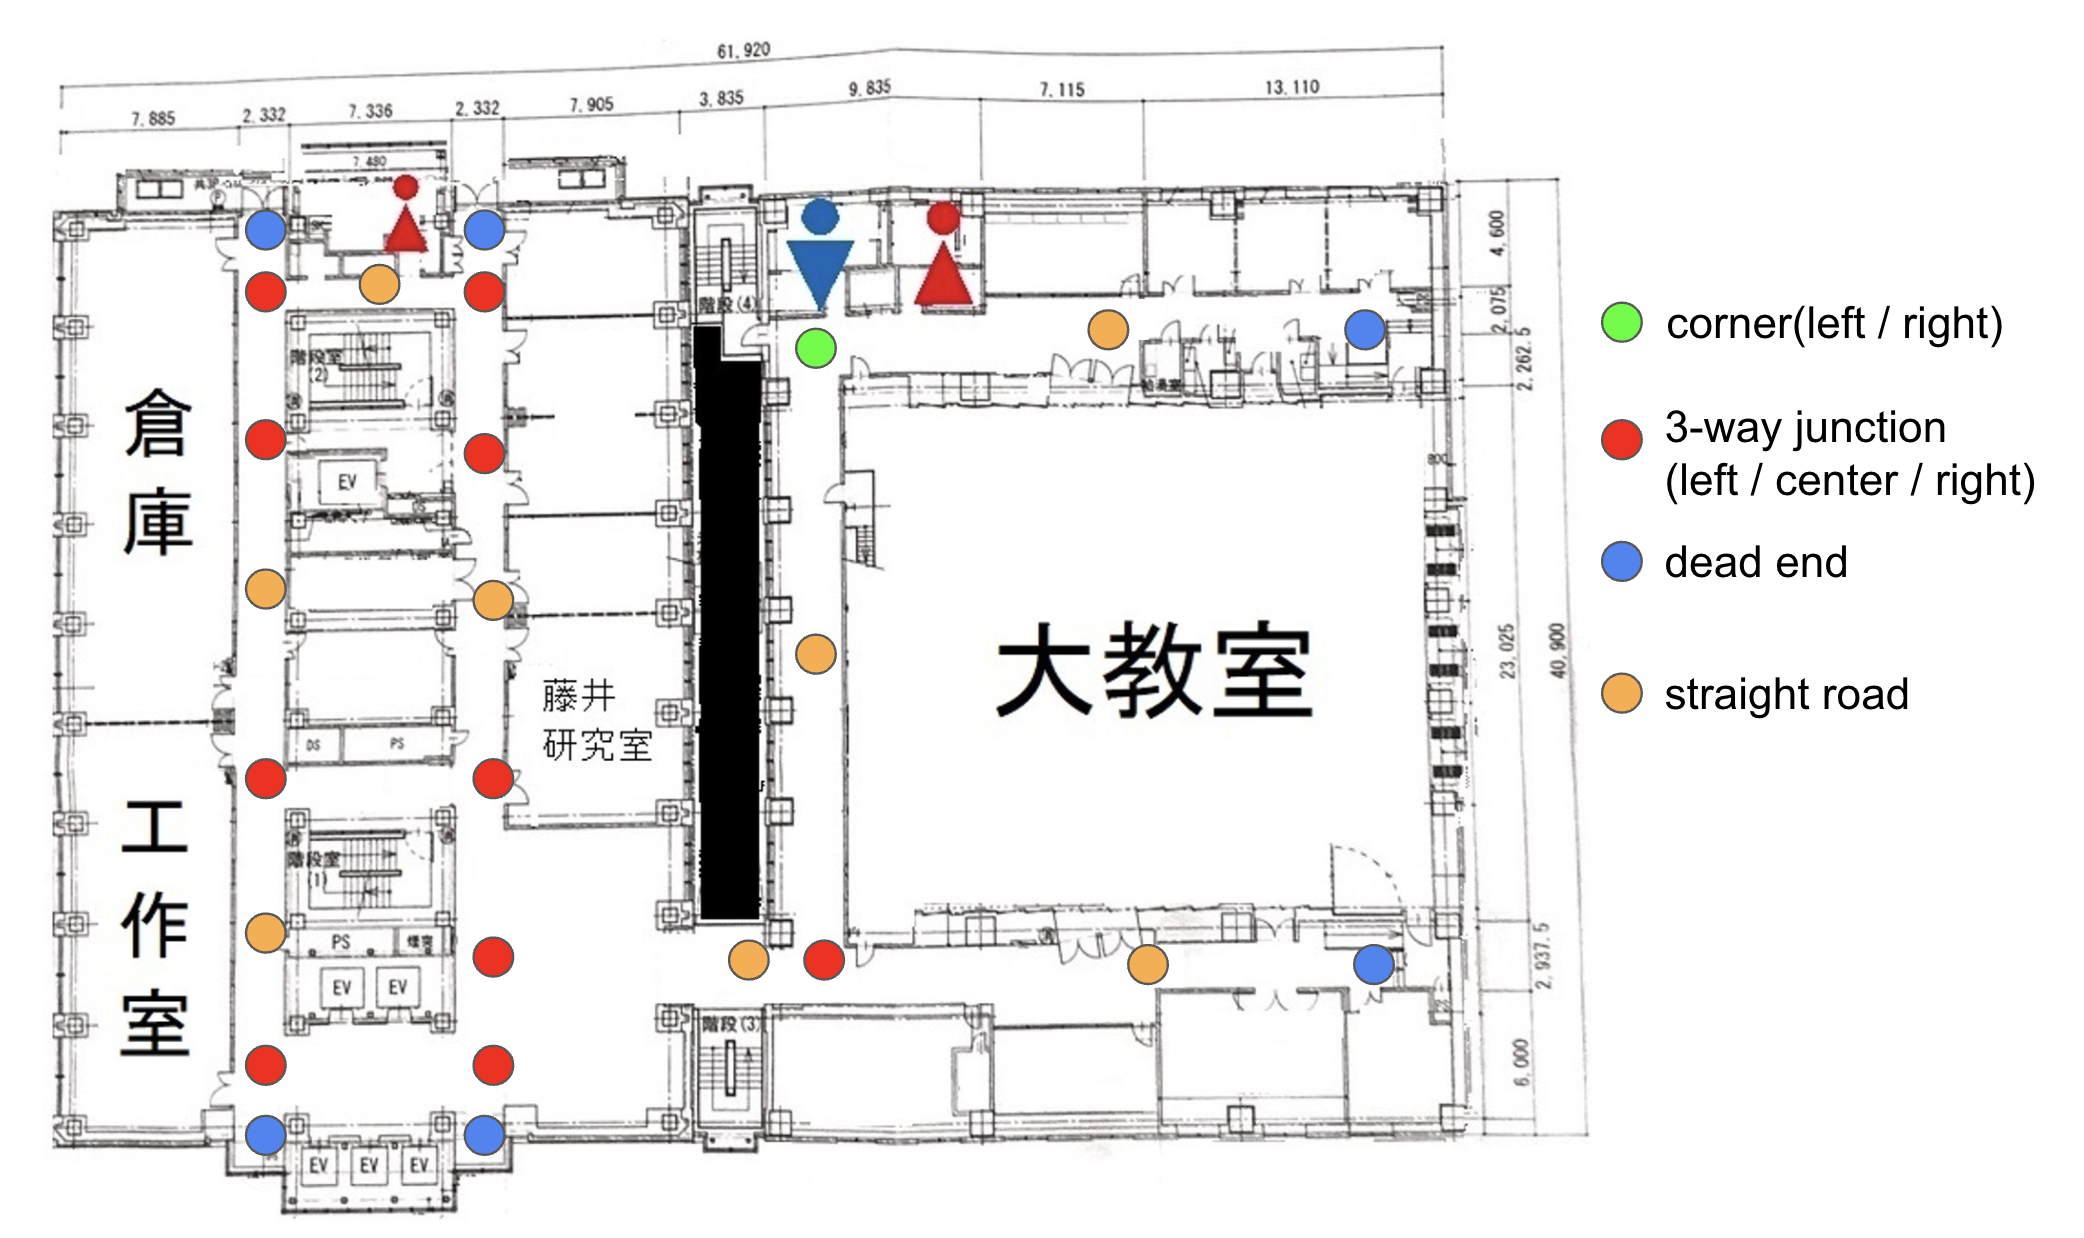
\includegraphics[width=20cm]{../images/experiment_point.png}
         \section{25 places to place robots in aisle classification experiments}
         \label{figure::experiment_point}
        \end{figure}

        \subsection{結果と考察}
        実験の結果.●例中●例で正しく通路の特徴を分類することができた.
        正しく分類ができた例の一部をFig~に示す.また,分類に失敗してしまった例の一部をFig〜に示す.
        今回,分類に失敗した原因として,○○ということが考えられる.
\end{document}